%miktex
\documentclass[conference]{IEEEtran}

\usepackage{graphicx,times,amsmath,colortbl, psfrag} % Add all your packages here

\usepackage[ruled, vlined, english, boxed, linesnumbered, lined]{algorithm2e} %descargar
\usepackage{algpseudocode} %descargar

\usepackage{multirow}

\usepackage {amsfonts}
\usepackage {amsmath}




% *** GRAPHICS RELATED PACKAGES ***
%
\ifCLASSINFOpdf
  % \usepackage[pdftex]{graphicx}
  % declare the path(s) where your graphic files are
   \graphicspath{{../pdf/}{../jpeg/}}
  % and their extensions so you won't have to specify these with
  % every instance of \includegraphics
   \DeclareGraphicsExtensions{.pdf,.jpeg,.png}
\else
  \fi


\begin{document}
%
% paper title
% can use linebreaks \\ within to get better formatting as desired
\title{Brief simulation report on "A Decoupling Scheme for Fore Control in Cooperative Multi-Robot Manipulation Tasks" by De Pascali, Erhart et al.}


% author names and affiliations
% use a multiple column layout for up to three different
% affiliations
\author{\IEEEauthorblockN{Martin Angerer}

\IEEEauthorblockA{
Master Student, ITR, TUM\\
martin.angerer@tum.de
}
}

% make the title area
\maketitle

\begin{abstract}
Purpose of the simulation is to evaluate the performance of the proposed \textit{desired internal force allocator} against the classic nullspace of the grasp matrix approach. In contrast to the simulations done by the authors four manipulators are used in a symmetric set-up. The results indicate that the internal force calculation proposed by De Pascali et al is only comprehensive for a 2-manipulator set-up. The \textit{desired internal force allocator} outperforms the nullspace-approach in terms of settling time, transient behaviour and harmonic distortion.
\end{abstract}

\section{Theory}
The geometry of a multi-robot cooperative manipulation set-up is described with the grasp matrix. The grasp matrix is used to render the manipulator's trajectories based on a desired object trajectory. Thus the manipulators should not exert internal stress on the object. In some applications (e.g. friction grasp) it is required to exert and control internal forces. Internal wrenches, which do not contribute to the object motion, lie in the null space of the grasp matrix. Therefore desired internal forces can be calculated by multiplying an arbitrary vector with the base of the null space of the grasp matrix. Pratically the vector is chosen to meet desired amount and direction of the internal forces.
De Pascali, Erhart et. al. propose to use an additional internal force allocator, to decouple motion-inducing- and internal forces. Key element of the allocator is the calculation of the interaction wrenches between the manipulators, to this purpose the object is virtually removed and only the constrained system of manipulators is considered. Calculation is done using the Gauss' principle of least constraint. The interaction wrenches between the manipulators can be seen as internal forces. Inputs for the allocator are both the desired internal $ h^{int,d} $ and the motion-inducing $ h^x $ wrenches:
\begin{equation}
h_w^{x} = \bar{A}^T(\bar{A}M^{-1}\bar{A}^T)^{-1}(\bar{b}-\bar{A}M^{-1}(h^{int,d}+h^x))
\end{equation}
The allocator calculates the interaction wrenches arising from the inputs not compatible with the constraints. Constraint violating in this case are the internal forces, both the desired ones and the possibly included in the motion-inducing wrench. Adding up the interaction wrenches to the motion-inducing wrench eliminates the internal components from the motion inducing wrench. To this end, internal and motion-inducing wrenches can be independently specified.\\
For motion-inducing wrench free of internal forces $ h_w^x = h^{int,d} $. Inserting the control law for $ h^w $ gives further insight:
\begin{multline}
\bar{b} - \bar{A}M^{-1}h^x = \bar{b}-\bar{A}M^{-1}(M\ddot{x}^d - D[\dot{x}-\dot{x}^d] - h^K(x,x^d)) =\\
= \bar{b} - \underbrace{\bar{A}M^{-1}MG^T}_{\substack{0_{6(N-1)\times6}}}\ddot{x}_o^d -\underbrace{\bar{A}M^{-1}Mb}_{\substack{\bar{b}}} + \underbrace{\bar{A}M^{-1}DG^T}_{\substack{0_{6(N-1)\times6}}}[\dot{x}_o - \dot{x}_o^d] + \\
+ \bar{A}M^{-1}h^K(x,x^d) = \bar{A}M^{-1}h^K(x,x^d) 
\end{multline}
This means that only the stiffness part is potentially constraint violating. Lacking mathematical evidence, simulations are done to estimate whether the stiffness contribution is generating internal wrench and under which circumstances. 
\section{Simulation}
The set-up consists of 4 manipulators symmetrically distributed. Simulations are always done with and without the allocator to visualize the appearance of internal forces.
\subsection{Equally distributed internal forces}  
The most classic case, the manipulators symmetrically exert internal force on the object. The object is moved in sinusoidal velocity curve in x-direction and with constant velocity in z-direction. It is rotated with constant angular velocity in y- and z- direction. Deviations occur in transient behaviour, changing velocity with a step (figure \ref{IntForceStep}) causes high internal forces in the allocator-free system. 
\begin{figure}
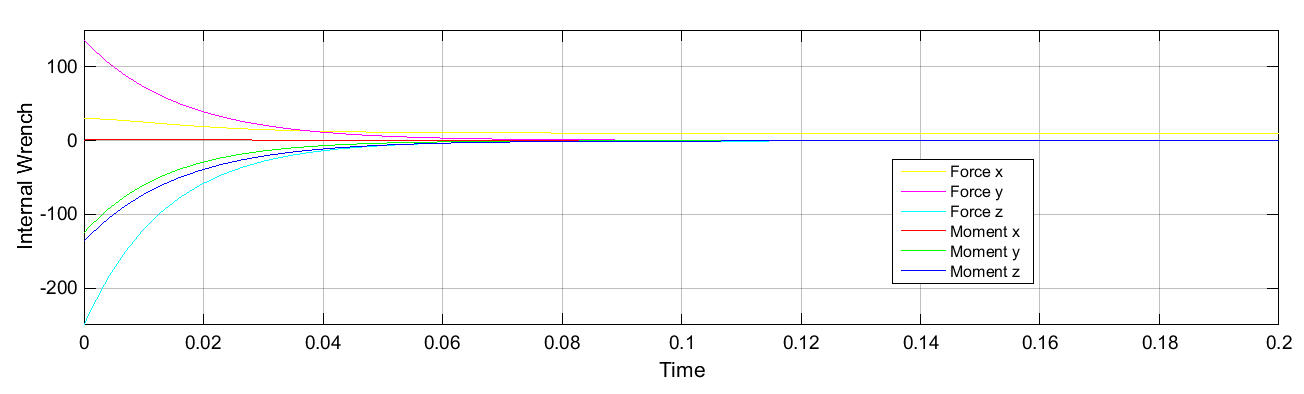
\includegraphics[width=\linewidth]{IntForceStep1}
\caption{Internal wrench for a step in velocity}
\label{IntForceStep}
\end{figure}
From figure \ref{IntForceRamp} it can be seen that limiting velocity rise decreases internal wrench significantly. Here a ramp function, which takes 10 ms to reach the prior step value is used.
\begin{figure}
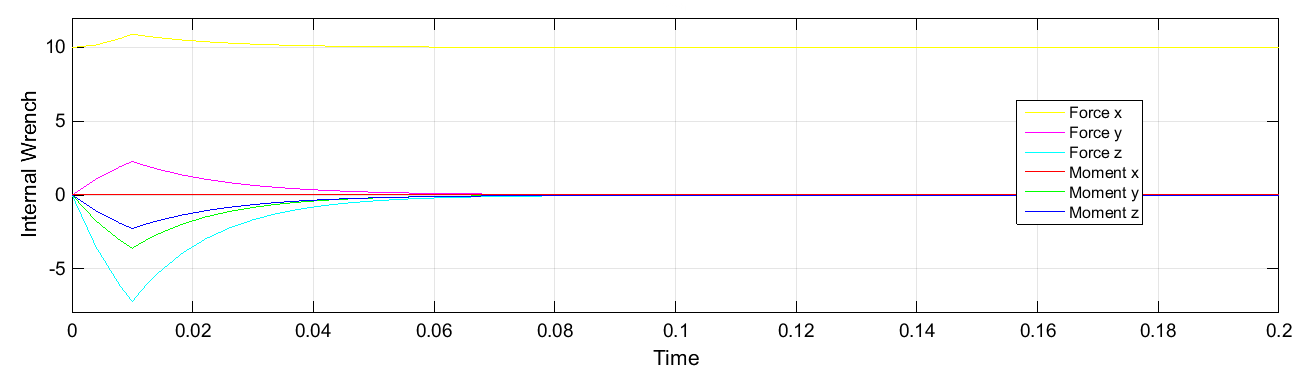
\includegraphics[width=\linewidth]{IntForceRamp1}
\caption{Internal wrench for ramping up velocity}
\label{IntForceRamp}
\end{figure}
In both cases the internal forces approach their desired values after some time. Using the allocator no difference between step and ramp can be noticed, the desired values are set immediately: wrenches in figure \ref{IntForceAllocator} are equal to the desired ones.
\begin{figure}
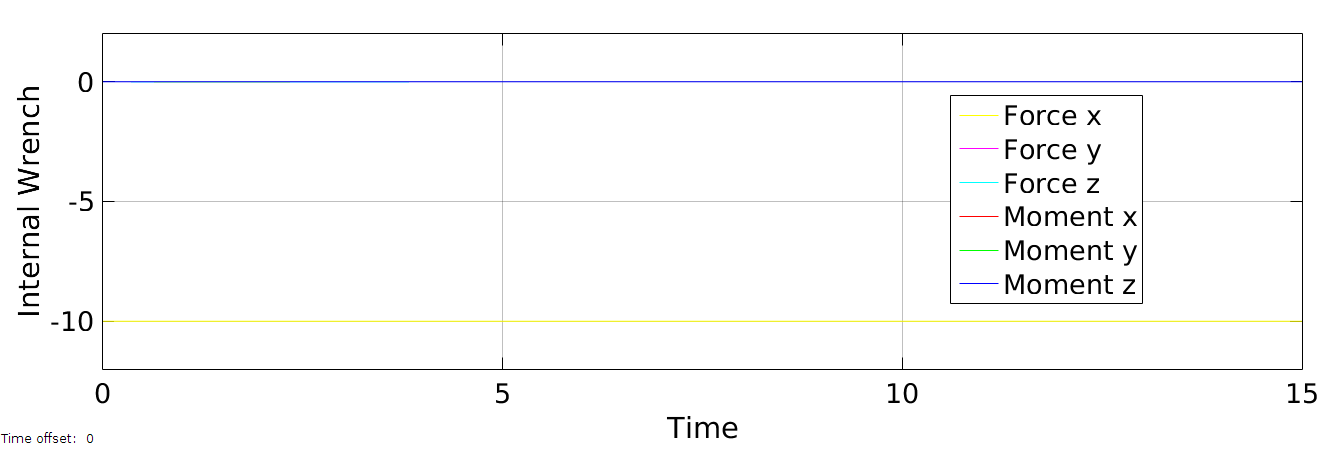
\includegraphics[width=\linewidth]{IntForceStepAllocator}
\caption{Internal wrench using the allocator}
\label{IntForceAllocator}
\end{figure}
Furthermore excluding the allocator results in some oscillations in the internal forces. Figure shows the internal force in x-direction, the other forces and moments have equal amplitude and frequency. This frequency of 0.225 \textit{Hz} is not influenced by model parameters (stiffness, damping, inertia, sinusoidal velocity in x-direction) and may thus be of numerical origin. The amplitude however increases with stiffness, decreases for higher damping and is almost constant for changes of inertia.




Key idea of the decoupling control scheme is using the internal force calculation presented by Erhart [??] to eliminate the internal components from motion inducing wrench and thus only obtaining the desired internal forces. Thereby decoupling between internal and motion inducing wrench is accomplished. In [??] the internal force calculation is based on virtually removing the object and thus only considering the forces exchanged between the manipulators. These forces are calculated using the Gauss' principle of least constraint. 

Cooperative manipulation systems are in general a set of \textit{N} manipulators rigidly connected to a rigid object. The rigid connections transmit both force and and are expressed by a number of kinematic constraints, \textit{$ m_{C} $}, which reduce the degrees of freedom (DOF) of the constrained system. Motion or the attempt to move in the constrained directions results in internal loading of the object. Therefore trajectories of the manipulators have to be generated to avoid internal stress on the object. In some applications internal forces on the object are desired, so that motion and internal forces are to be controlled independently.
Impedance control is a well known strategy to avoid unbounded forces when it comes to interaction of manipulators with objects/environment. The policy does not control one state variable (e.g. position, velocity, force) but enforces a relation between them. The impedance control scheme can be described as a spring- damper- mass system.
\begin{equation}
M\Delta\ddot{x} + D\Delta\dot{x} + K\Delta x = h
\end{equation}
Where \textit{M,D,K} can be arbitrarily chosen.


\section{Selected work}
Selected work which contribute to the problem of cooperative manipulation are presented in the following. This will be done chronologically.


\subsection{Schneider, Cannon, "Object Impedance Control for Cooperative Manipulation: Theory and Experimental Results", 1992}

An object focussed approach, the motion of the object is controlled and the object itself is being replaced by a "virtual object". The object is now a controlled impedance, which interacts with the environment via a set of damped springs. They are positioned at the virtual centre of mass and they are orthogonal, they connect to the environment in selectable points. The control law is
\begin{equation}
m_d(\ddot{x}-\ddot{x}_d) + k_v(\dot{x}-\dot{x}_d) + k_p(x-x_d) = f_{ext}
\end{equation}
Where \textit{x} is the one degree of freedom. \textit{$ x_d $} is the reference signal, $ \ddot{x}_d $ denotes the feed forward desired acceleration. $ \ddot{x} $ is the control output. Deviations from the desired trajectory due to the external force/moment $ f_{ext} $ are corrected by the impedance relation.

The object's equations of motion are 
\begin{multline}
\begin{bmatrix}mI_3 & mR \\0_3 & I\end{bmatrix}
\begin{bmatrix}\ddot{\textbf{y}}\\\dot{\boldsymbol{\omega}}\end{bmatrix} + 
\begin{bmatrix}-m\boldsymbol{g}-m(\boldsymbol{\omega} \times (\boldsymbol{\omega} \times \boldsymbol{r}))\\\boldsymbol{\omega} \times I \boldsymbol{\omega}\end{bmatrix}\\
=\begin{bmatrix}\textbf{\textit{f}}_{ext}\\\boldsymbol{\tau}_{ext}\end{bmatrix}+
\begin{bmatrix}\sum\textbf{\textit{f}}_i\\\sum\textit{\textbf{p}}_i \times \textit{\textbf{f}}_i + \sum\textit{\textbf{m}}_i\end{bmatrix}
\end{multline}
and written more compactly
\begin{equation}\label{actualobjectimpedance}
I_0\ddot{Y}+B_0 = \textbf{\textit{F}}_{ext}+W\textbf{\textit{F}}
\end{equation}
\textit{W} denotes the grasp matrix. \\
The controller specifies a desired object behaviour to a external force
\begin{equation}
\begin{bmatrix}M_d & 0_3 \\0_3 & I_d\end{bmatrix}
\begin{bmatrix}\ddot{\textbf{y}}\\\dot{\boldsymbol{\omega}}\end{bmatrix} + 
\begin{bmatrix}0\\\boldsymbol{\omega} \times I_d \boldsymbol{\omega}\end{bmatrix}
=\begin{bmatrix}\textbf{\textit{f}}_{ext}\\\boldsymbol{\tau}_{ext}-\textbf{\textit{r}}\times\textbf{\textit{f}}_{ext}\end{bmatrix}
\end{equation}
What again can be rewritten more compact
\begin{equation}
I_{0d}\ddot{Y}+B_{0d} = \textbf{\textit{\~{F}}}_{ext}
\end{equation}
This gives directly the desired acceleration of the virtual object
\begin{equation}
\ddot{Y}_{cmd} = I_{0d}^{-1}(\textbf{\textit{\~{F}}}_{ext}-B_{0d})
\end{equation}
This output of the object impedance controller is now reinserted in the actual object dynamics equation (\ref{actualobjectimpedance}) to calculate the required wrench.
\begin{equation}
\textbf{\textit{F}}_{cmd} = W^{wpi}(B_0-\textbf{\textit{F}}_{ext}+I_0I_{0d}^{-1}(\textbf{\textit{\~{F}}}_{ext}-B_{0d})) + \textbf{\textit{F}}_{int}
\end{equation}
$ W^{wpi} $ is a weighted pseudoinverse of the grasp matrix. With $ \textbf{\textit{F}}_{int} $ an internal force can be added, but there is no closed force feedback loop.
To complete the control loop the desired joint accelerations are computed via the inverse Jacobian. At the point of calculating the joint torques, the manipulator's dynamics are considered
\begin{equation}
\boldsymbol{\tau}_i = M_i\ddot{\textbf{\textit{q}}}_{i_{cmd}} + C_i(\textbf{\textit{q}},\dot{\textbf{\textit{q}}}) + J_i^T(\textbf{\textit{F}}_{i_{cmd}})
\end{equation}
Finally $ \textbf{\textit{F}}_{ext} $ has to be derived, this is done using (\ref{actualobjectimpedance}) with an estimate of $ \ddot{Y} $.
\\
\emph{Conclusion: }This pioneer work introduces a object impedance control scheme in operational space. The object trajectory is corrected w.r.t. to external forces. Dynamics of object and manipulators are compensated. An impedance relation between object and manipulators is not enforced, internal forces on the object can be set but are not regulated. The dynamic properties of the object have to be known.

%%%%%%%%%%%%%%%%%%%%%%%%%%%%%%%%%%%%%%%%%%%%%%%%%%

\subsection{Bonitz, Hsia, "Internal Force Based Impedance Control for Cooperating Manipulators", 1996}
This work is going without knowledge of the dynamics of the object. The manipulators are given impedance properties and a relation between velocity and internal force is established. This is done in order to improve tracking and prevent position errors, due to unknown dynamics of the object. If the total forces exerted by the object on the manipulators were incorporated in the impedance control, it would lead to a deviation. Therefore the impedance control law is
\begin{equation}
M_i\Delta\ddot{\textbf{\textit{x}}} + B_i\Delta\dot{\textbf{\textit{x}}} + K_i\Delta\textbf{\textit{x}} = \Delta\textbf{\textit{h}}_{Ii}
\end{equation}
$ M_i, B_i, K_i $ are the desired inertia, damping and stiffness matrices of the i-th robot.\\ $ \Delta\textbf{\textit{x}} = \textbf{\textit{x}}_d - \textbf{\textit{x}}  $ is the position and orientation error of the i-th end-effector in task space.\\ $ \Delta\textbf{\textit{h}}_I = \textbf{\textit{h}}_{Id} - \textbf{\textit{h}}_I $ is the internal wrench error at the i-th robot.\\
Similarly to the previous section the output acceleration can be inserted in the actual dynamic equation to compute the necessary wrench. The joint torque of the i-th manipulator is
\begin{multline}
\boldsymbol{\tau}_i = D_i \{ J_i^{-1} ( M_i^{-1} [M_i\ddot{\textbf{\textit{x}}}_id + B_i\Delta\dot{\textbf{\textit{x}}} + K_i\Delta\textbf{\textit{x}} - \Delta\textbf{\textit{h}}_{Ii}] - \dot{J}_i\dot{\textbf{\textit{q}}}_i) \}\\ + E_i + J_i^T\textit{\textbf{h}}_i
\end{multline}
$ D_i $ is the actual inertia of the i-th robot. $ E_i $ is the combined Coriolis, centripetal and gravity vector. $ \textbf{\textit{h}}_{Iid} $ is calculated from the measured wrench using the null space projection of the grasp matrix.\\
On the input side, desired trajectories are specified for the object. They are mapped to the manipulators, compliant with the grasp geometry.\\
\emph{Conclusion: }The interaction of manipulator and object is controlled. With the impedance relation between velocity and internal forces separate control loops for force and position are not necessary. Internal force can be specified and is regulated. The approach is operational space based and knowledge of the object dynamics is not necessary. 

%%%%%%%%%%%%%%%%%%%%%%%%%%%%%%%%%%%%%%%%%%%%%%

\subsection{Caccavale, Villani, "An Impedance Control Strategy for Cooperative Manipulation", 2001}
This work promises to  combine the previously presented  two attempts to control first the interaction forces between environment and object and second the relation between object and manipulator. Object and manipulators are both subject to impedance control. Compliant behaviour is enforced between manipulator and object and the trajectory is modified w.r.t to external forces. The unit quaternion for expressing orientation is introduced. The control strategy consists of a inner motion control loop and a outer position control loop. The inner loop is designed to guarantee tracking of a reference end- effector position and orientation. Therefore an inverse dynamics strategy is adopted for linearising and decoupling of the links. The joint torques are
\begin{equation}
\boldsymbol{\tau}_i = M_i  J_i^{-1} ( \textbf{\textit{a}}_i - \dot{J}_i\dot{\textbf{\textit{q}}}_i) + C_i\dot{\textbf{\textit{q}}}_i + \textbf{\textit{g}}_i +  J_i^T\textbf{\textit{h}}_i
\end{equation}
$ M_i,C_i $ are the inertia and Coriolis matrices, $ \textbf{\textit{g}}_i,\textbf{\textit{h}}_i $ are the gravity and wrench, acting at the i-th end effector, vectors.
$ \textbf{\textit{a}}_i $ is a new control input.
\begin{equation}
\textbf{\textit{a}}_i = \ddot{\textbf{\textit{x}}}_{i_r} + k_v(\dot{\textbf{\textit{x}}}_{i_r} - \dot{\textbf{\textit{x}}}_{i}) + k_P(\textbf{\textit{x}}_r - \textbf{\textit{x}})
\end{equation}
$ \textbf{\textit{x}}_r,\textbf{\textit{x}} $ denoting the reference and actual stacked vectors of position and orientation. \\
An impedance relation between object and environemnt is used to generate a reference object trajectory from the desired object trajectory:
\begin{equation}
\boldsymbol{\alpha}M_o(\ddot{\textbf{\textit{x}}}_{o_d} - \ddot{\textbf{\textit{x}}}_{o_r})  + D_o(\dot{\textbf{\textit{x}}}_{o_d} - \dot{\textbf{\textit{x}}}_{o_r}) + K_o(\textbf{\textit{x}}_{o_d} - \textbf{\textit{x}}_{o_r})  = \textbf{\textit{h}}_{env}
\end{equation}
where $ M_o $denotes the actual object inertia matrix, $ \boldsymbol{\alpha} $ is a positive constant to be chosen. $ D_o, K_o $ are the tunable damping and stiffness matrices. $ \textbf{\textit{x}}_{o_d} $ along with its derivatives is the control input. The wrench exerted by the object on the environment is calculated:
\begin{equation}
\textbf{\textit{h}}_{env} = \textbf{\textit{h}}_{e} +m_0\textbf{\textit{g}} - M_o\ddot{\textbf{\textit{x}}}_{o_r}
\end{equation}
$ \textbf{\textit{h}}_e $ is the wrench exerted by the manipulators on the object. Control output is the reference acceleration of the object $ \ddot{\textbf{\textit{x}}}_{o_r} $. With the geometry of the grasp, the inputs $ \textbf{\textit{x}}_{i_d}, \dot{\textbf{\textit{x}}}_{i_d}, \ddot{\textbf{\textit{x}}}_{i_d}  $ of the manipulator/ object impedance controller can be determined. Similar to the former section the impedance relation is enforced between end effector displacement and internal force
\begin{equation}
M_I(\ddot{\textbf{\textit{x}}}_{i_d} - \ddot{\textbf{\textit{x}}}_{i_r})  + D_I(\dot{\textbf{\textit{x}}}_{i_d} - \dot{\textbf{\textit{x}}}_{i_r}) + K_I(\textbf{\textit{x}}_{i_d} - \textbf{\textit{x}}_{i_r})  = \textbf{\textit{h}}_{Ii}
\end{equation}
No desired internal wrench is included in this approach but can easily be added. The reference acceleration $ \ddot{\textbf{\textit{x}}}_{i_r} $ is the control output and along with its integrals the input for the inner motion control loop. \\
\emph{Conclusion: } The overall control scheme consists of three levels: an inner motion controller of PD- structure with acceleration feed-forward. With inverse dynamics control it compensates for the manipulator- dynamics. Superimposed is a impedance controller for the manipulator/object relation which corrects the reference trajectories if internal forces are present and therefore allows high gains in the inner motion loop. The highest level is the impedance controller for environment/object behaviour, it ensures object-compliance w.r.t external forces. All controllers are realized in operational space. Inertia of the object has to be known.

%%%%%%%%%%%%%%%%%%%%%%%%%%%%%%%%%%%%%%%%%%%%%%%%%%%%%%%%%%%%%%%

\subsection{Caccavale, Chiacchio, et al., "Six-DOF Impedance od Dual-Arm Cooperative Manipulators", 2008}
The work is very similar to the former. The overall control scheme is equal, in the inner motion control loop the inverse dynamics controller is replaced by an PID one. This is due to the wide distribution of PID controller in industrial robots, with which the experimental part of the work is carried out.\\
The main contribution of the work is extending the \emph{geometrically consistent stiffness} to the case of finite displacements. Moreover the presented concept allows to specify direction dependent stiffness.\\
The experimental results show good performance also in the case of non-rigid objects.

%%%%%%%%%%%%%%%%%%%%%%%%%%%%%%%%%%%%%%%%%%%%%%%%%%%%%%%%%%%

\subsection{Erhart, Hirche, "Model and analysis of the interaction dynamics in cooperative manipulation tasks", 2014}
This work is confined to task space considerations, only the end-effector dynamics are viewed by assuming perfect linearisation and decoupling of the subjacent manipulator structure. Moreover in this way actual manipulator-dynamics can be replaced by a desired second-order impedance behaviour:
\begin{equation}
M_i[\ddot{x}_i - \ddot{x}_i^d] + D_i[\dot{x}_i - \dot{x}_i^d] + h_i^K(x_i,x_i^d) = h_i - h_i^d
\end{equation}
$ x_i $ denotes the stacked position and orientation vector, $ h_i $ the end-effector wrench of the i-th manipulator.The inertia, $ M_i $, and Damping, $ D_i $, matrices are block-diagonal, decoupling translational and rotational behaviour. The term $ h_i^K(x_i,x_i^d) $ is the \textit{geometrically consistent stiffness} and is similarly defined to the former. Stiffness is considered to be isotropic, i.e. there is no coupling between the single DOF. \\
Lagrange formulation of the object dynamics is:
\begin{equation}
M_o \ddot{x}_o + C_o\dot{x}_o + h_g = h_o
\end{equation}
$ M_o, C_o, h_g $ are the object's inertia, centripetal force and gravity parameters. \\
The kinematic constraints impose additional forces of interaction on the system. Both manipulator and object dynamics can be re-formulated to distinguish between a local or non-interacting wrench and a global or interacting wrench. 
\begin{equation}
	M_i \ddot{x}_i  = h_i^\Sigma + h_i
\end{equation}
\begin{equation}
M_o \ddot{x}_o  = h_o^\Sigma + h_o
\end{equation}
Where $ h_i^\Sigma = M_i\ddot{x}_i^d - D_i[\dot{x}_i - \dot{x}_i^d] - h_i^K(x_i,x_i^d) $ and  $ h_o^\Sigma = -C_o\dot{x}_i^d - h_g $. The equations of the complete system can be written as
\begin{equation}
M \ddot{x} = h^\Sigma + h
\end{equation}
with $ M = blkdiag(M_o,M_1,...,M_N) $, $ h^\Sigma = (h_o^\Sigma;h_1^\Sigma;...;h_N^\Sigma) $ and $ h = (h_o;h_1;...;h_N) $
The rigid grasp kinematic constraints can be formulated in matrix- vector notation:
\begin{equation}
A \ddot{x} = b
\end{equation}
Employing \textit{Gauss principle of the least constraint} an explicit solution for $ h $ be found: 
\begin{equation}
h = M^{\frac{1}{2}}(AM^{-\frac{1}{2}})^{\dagger}(b - AM^{-1}h^\Sigma)
\end{equation}
Where $ \dagger $ denotes the \textit{Moore-Penrose generalized inverse} \cite{UdwadiaKalaba1992}.\\
To address asymmetric load distributions the paper proposes a specific weighted generalized inverse of the grasp matrix for manipulator coordination.\\
Concluding the system description an overall impedance of the constrained system is formulated,which is effective when it comes to disturbances acting on the object. \\
The paper proposes to calculate the internal force acting on the object via a reduced system consisting of constrained manipulators without the object. Therefore the reduced kinematic constraints are $ A'\ddot{x}' = b' $. $ \ddot{x}' = [x_1^T,...,x_N^T]^T $ is the stacked vector of position and orientation of the $ N $ manipulators. Consequently $ A' $ is the $ 6N $ identity matrix. With $ b' = b = [(S(\omega_0)^2r_1)^T,0_{3\times1},...,(S(\omega_o)^2r_N)^T,0_{3\times1} ]^T $ the accelerations consistent with the constraints are $ \ddot{x}' = b $. The proposed calculation of the internal force is
\begin{equation}
h'_{int} = M'^{\frac{1}{2}}(A'M'^{-\frac{1}{2}})^{\dagger}(b' - A'M'^{-1}h'^{\Sigma})
\end{equation}
with the commanded acceleration vector $ \ddot{x}'^x $. Computing this equation one obtains:
\begin{multline}
h'_{int} = [(M_1S(\omega_0)^2r_1 - f_1^\Sigma)^T,(-t_1^\Sigma)^T,...,\\,(M_NS(\omega_0)^2r_N - f_N^\Sigma)^T,(-t_N^\Sigma)^T]^T
\end{multline}
With $ f_*,t_* $ being the force and torque vectors exerted by the manipulators.
Apart from the centripetal force, the internal forces are just the opposite of the wrench exerted by the manipulators. One gets the same result using Newton's third law.
Thus every attempt changing the dynamic state of the object, i.e. accelerating the object, leads to internal loading. \\
\textit{Conclusion:} In terms of control architecture, the key idea presented in this work is replacing the actual dynamic properties of the manipulators by a desired mechanical impedance. The rest of the paper is modeling the constrained system: an explicit solution for the constraining wrenches is given. The constrained system response to disturbances is formulated. A (complicated) solution for calculation internal forces is presented. The proposed plant model is exploited for control design in the next section. 

%%%%%%%%%%%%%%%%%%%%%%%%%%%%%%%%%%%%%%%%%%%%%%%%%

\subsection{De Pascali, Erhart, et al., "A Decoupling Scheme for Force Control in Cooperative Multi-Robot Manipulation Tasks", 2015}

Although partially written by the same authors than the former, this work comes up with another new calculation method for the internal forces. They are defined as the forces/torques which do not produce virtual work for a virtual displacement compliant with the kinematic constraints. Geometrically spoken this means that internal forces/torques are orthogonal to the kinematic constraints. Internal wrench calculation starts from re-formulating the kinematic constraints for the relative position/orientation of the end-effectors. This is done by subtracting the dynamics equations of the i-th manipulator from the j-th manipulator. This eliminates the dynamics of the object from the formulation. The relative position is $ \Delta r_{ji} = r_j-r_i $. The resulting constraint matrix is: 
\begin{equation}
\bar{A} =
\begin{bmatrix}
-I_3 & S(\Delta r_{21}) & I_3 & 0_3 & & &\\
0_3 & -I_3 & 0_3 & I_3 & & &\\
\vdots & \vdots & & & \ddots & & \\
-I_3 & S(\Delta r_{N1}) & & & & I_3 & 0_3\\
0_3 & -I_3 & & & & 0_3 & I_3
\end{bmatrix}
\end{equation}
The basis of the nullspace of the grasp matrix $ G $ is $ \bar{A}^T $. This is equal to $ Ker(G)\equiv Im(\bar{A}^T) $, what is shown in the paper. The internal wrench is calculated as
\begin{equation}
h^{int} = \bar{A}^T(\bar{A}M^{-1}\bar{A}^T)^{-1}(\bar{b}-\bar{A}M^{-1}\bar{h}^{\Sigma})
\end{equation}
Where $ M = blkdiag(M_1,...,M_N) $.
It is shown that $ h^{int} \in ker(G) $, i.e. it does not influence motion. On the other hand it is shown that a commanded object motion mapped to the manipulators using $ G $ does not generate internal wrench. Just as in the previous section, the motion control law is: 
\begin{equation}
M_i[\ddot{x}_i - \ddot{x}_i^d] + D_i[\dot{x}_i - \dot{x}_i^d] + h_i^K(x_i,x_i^d) = h_i - h_i^d
\end{equation}
Another re-formulation is introduced:
\begin{equation}
M\ddot{x} = h^x + h^d + h
\end{equation}
Where $ h^x $ accounts for the local end-effector dynamics, $ h^d $ can be seen as a feed-forward term of the desired object acceleration, $ h $ is again the interaction wrench. Note that in this work the stacked vector $ h = [h_1^T,...,h_N^T]^T $ excludes the wrench acting on the object. $ h^d $ is calculated from $ h_o^d $ with a non-squeezing pseudo-inverse $ G_M^+ $ of the grasp matrix. The desired velocity $ \dot{x}^d $ is calculated with the transposed grasp matrix $ G^T $.  The control law to render the internal forces is
\begin{equation}
h_w^{x} = \bar{A}^T(\bar{A}M^{-1}\bar{A}^T)^{-1}(\bar{b}-\bar{A}M^{-1}(h^{int,d}+h^x))
\end{equation}
Interestingly, next to the desired internal forces $ h^{int,d} $, the impedance control output of the manipulators $ h^x $ is incorporated in the internal force allocation. Vice versa this means that $ h^x $ is not free of internal force components. $ h^{int,d} = \bar{A}^Tz$ is calculated to lie in the null space of the grasp matrix. Recall that $ \bar{A}^T $ is the basis of the null space of $ G $. If $ h^x $ would be free of internal wrench, then $ \bar{A}^Th^x = 0_{6N\times1} $.
\begin{multline}
\bar{b} - \bar{A}M^{-1}h^x = \bar{b}-\bar{A}M^{-1}(M\ddot{x}^d - D[\dot{x}-\dot{x}^d] - h^K(x,x^d)) =\\
= \bar{b} - \underbrace{\bar{A}M^{-1}MG^T}_{\substack{0_{6(N-1)\times6}}}\ddot{x}_o^d -\underbrace{\bar{A}M^{-1}Mb}_{\substack{\bar{b}}} + \underbrace{\bar{A}M^{-1}DG^T}_{\substack{0_{6(N-1)\times6}}}[\dot{x}_o - \dot{x}_o^d] + \\
+ \bar{A}M^{-1}h^K(x,x^d) = \bar{A}M^{-1}h^K(x,x^d) 
\end{multline}
There are two possibilities: 1. the \textit{geometrically consistent stiffness} term produces internal wrench or 2. it does not and the author is just incapable of proofing $ \bar{A}M^{-1}h^K(x,x^d) = 0_{6(N-1)\times1} $. If 2. is true then $ h^x_w = \bar{A}^Tz = h^{int,d} $, in account with previous literature.\\
Finally the resulting object acceleration is derived:
\begin{equation}
\ddot{x}_o = (M_o + GMG^T)^{-1}(h_o^{\Sigma} + G(h^x + h_w^x + h^d) - GMb)
\end{equation}

%%%%%%%%%%%%%%%%%%%%%%%%%%%%%%%%%%%%%%%%%%%%%%%%%%%%%%

\subsection{Wimbck, Ott, et al.,"Comparison of object-level grasp controllers for dynamic dextrous manipulation", 2011}


\section{Conclusions}


%\bibliography{my-paper}


% (used to reserve space for the reference number labels box)
\begin{thebibliography}{1}

\bibitem{UdwadiaKalaba1992}
Udwadia F. and Kalaba R.,
\newblock {"A new perspective on constrained motion",}
\newblock  \textit{Proceedings: Mathematical and Physical Sciences}, vol. 439, no. 1906, pp. 407 - 410, 1992



\end{thebibliography}




% that's all folks
\end{document}


